\documentclass[crop,tikz,convert={size=512x512,outext=.png}]{standalone}
\usetikzlibrary{shapes.geometric}
\begin{document}
  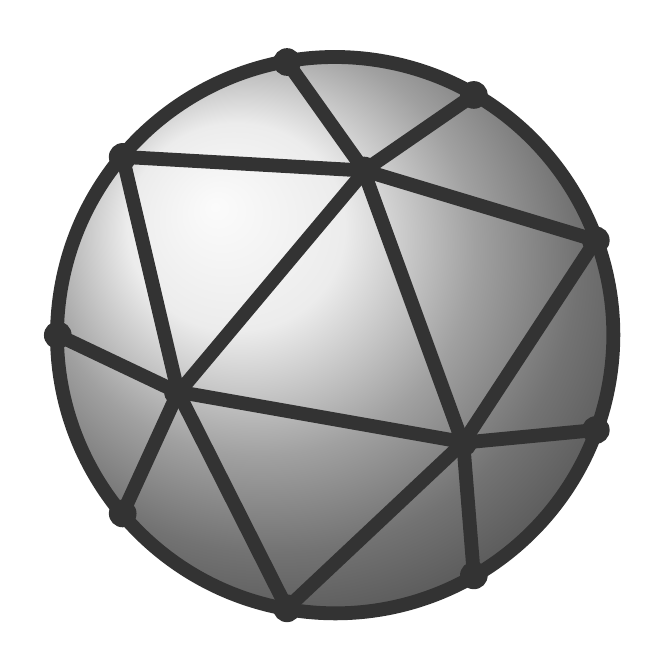
\begin{tikzpicture}
    [linestyle/.style={draw=black!80,line width=5pt,transform shape},
     emptylinestyle/.style={transform shape},
     circlestyle/.style={fill=black!80,circle,minimum size=10pt}]

    \begin{scope}[rotate=-10]
    \shadedraw [shading=ball, ball color=black!10] (0,0) circle (101pt);

    \node[linestyle,circle,minimum size=201pt] {};
    \node[emptylinestyle,regular polygon, regular polygon sides=9,rotate=20, minimum size=200pt] (p) {};
    \node[emptylinestyle, regular polygon, regular polygon sides=3,minimum size=120pt] (t) {};
    \node[linestyle, regular polygon, regular polygon sides=3,minimum size=120pt] {};

    \draw [linestyle] (t.corner 1) -- (p.corner 1);
    \draw [linestyle] (t.corner 1) -- (p.corner 2);
    \draw [linestyle] (t.corner 1) -- (p.corner 8);
    \draw [linestyle] (t.corner 1) -- (p.corner 9);
    \draw [linestyle] (t.corner 2) -- (p.corner 2);
    \draw [linestyle] (t.corner 2) -- (p.corner 3);
    \draw [linestyle] (t.corner 2) -- (p.corner 4);
    \draw [linestyle] (t.corner 2) -- (p.corner 5);
    \draw [linestyle] (t.corner 3) -- (p.corner 5);
    \draw [linestyle] (t.corner 3) -- (p.corner 6);
    \draw [linestyle] (t.corner 3) -- (p.corner 7);
    \draw [linestyle] (t.corner 3) -- (p.corner 8);

    \node [circlestyle] at (t.corner 1) {};
    \node [circlestyle] at (t.corner 2) {};
    \node [circlestyle] at (t.corner 3) {};
    \node [circlestyle] at (p.corner 1) {};
    \node [circlestyle] at (p.corner 2) {};
    \node [circlestyle] at (p.corner 3) {};
    \node [circlestyle] at (p.corner 4) {};
    \node [circlestyle] at (p.corner 5) {};
    \node [circlestyle] at (p.corner 6) {};
    \node [circlestyle] at (p.corner 7) {};
    \node [circlestyle] at (p.corner 8) {};
    \node [circlestyle] at (p.corner 9) {};
    \end{scope}
  \end{tikzpicture}
\end{document}
